\documentclass{standalone}
\usepackage{tikz}
\tikzset{cross/.pic = {  \draw[rotate = 45] (-#1,0) -- (#1,0);
                         \draw[rotate = 45] (0,-#1) -- (0, #1);}}
\begin{document}
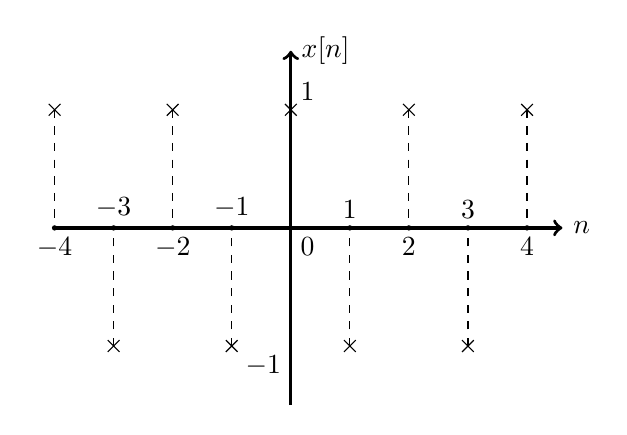
\begin{tikzpicture}[scale=1.5]
    \draw[->,very thick](0,-1.5)--(0,1.5)node[right]{$x[n]$};
        \draw[->,very thick](-2,0)--(2.3,0)node[right]{$n$};   
     
        \draw (0,1)pic[black]{cross=3pt};
        \draw (0.5,-1)pic[black]{cross=3pt};
        \draw (-0.5,-1)pic[black]{cross=3pt};
        \draw (1,1)pic[black]{cross=3pt};
        \draw (-1,1)pic[black]{cross=3pt};
        \draw (1.5,-1)pic[black]{cross=3pt};
        \draw (-1.5,-1)pic[black]{cross=3pt};
        \draw (2,1)pic[black]{cross=3pt};
        \draw (-2,1)pic[black]{cross=3pt};
        \draw[dashed](0.5,-1)--(0.5,0)node[above]{$1$};
        \draw[dashed](-0.5,-1)--(-0.5,0)node[above]{$-1$};
        \draw[dashed](1,1)--(1,0)node[below]{$2$};
        \draw[dashed](-1,1)--(-1,0)node[below]{$-2$};
        \draw[dashed](1.5,-1)--(1.5,0)node[above]{$3$};
        \draw[dashed](-1.5,-1)--(-1.5,0)node[above]{$-3$};
        \draw[dashed](2,1)--(2,0)node[below]{$4$};
        \draw[dashed](-2,1)--(-2,0)node[below]{$-4$};

        \filldraw[black](0.5,0)circle(0.5pt);
        \filldraw[black](-0.5,0)circle(0.5pt);
        \filldraw[black](1,0)circle(0.5pt);
        \filldraw[black](-1,0)circle(0.5pt);
        \filldraw[black](1.5,0)circle(0.5pt);
        \filldraw[black](-1.5,0)circle(0.5pt);
        \filldraw[black](2,0)circle(0.5pt);
        \filldraw[black](-2,0)circle(0.5pt);

        \node[above right]at(0,1){$1$};
        \node[below left]at(0,-1){$-1$};
        \node[below right]at(0,0){$0$};
\end{tikzpicture}
\end{document}